% chapter4.tex
% abx

%% Macros
\def\reals{\mathbb{R}}
\def\be{\begin{equation}}
\def\ee{\end{equation}}
\def\bea{\begin{eqnarray}}
\def\eea{\end{eqnarray}}
\def\bml{\begin{mathletters}}
\def\eml{\end{mathletters}}
\def\bse{\begin{subequations}}
\def\ese{\end{subequations}}
\def\expec{\mathbb{E}}
\def\exp{\text{exp}}
\def\Var{\text{Var}}
\def\e{\text{e}}
\def\ba{\begin{align}}
\def\ea{\end{align}}

\chapter{Sublethal antibiotics collapse gut bacterial populations by enhancing aggregation and expulsion}


Antibiotics induce large and highly variable changes in the intestinal microbiome even at sublethal concentrations, through mechanisms that remain elusive. Using gnotobiotic zebrafish, which allow high-resolution examination of microbial dynamics, we found that sublethal doses of the common antibiotic ciprofloxacin cause severe drops in bacterial abundance. Contrary to conventional views of antimicrobial tolerance, disruption was more pronounced for slow-growing, aggregated bacteria than for fast-growing, planktonic species. Live imaging revealed that antibiotic treatment promoted bacterial aggregation and increased susceptibility to intestinal expulsion. Intestinal mechanics therefore amplify the effects of antibiotics on resident bacteria. Microbial dynamics are captured by a biophysical model that connects antibiotic-induced collapses to gelation phase transitions in soft materials, providing a framework for predicting the impact of antibiotics on the intestinal microbiome.












\section*{Introduction}


    Antibiotic drugs induce large, long-lasting, and disease-associated alterations in the composition of the intestinal microbiota \cite{dethlefsen2011incomplete,cho2012antibiotics,schulfer2019impact}. Even at concentrations well below the minimum inhibitory levels of many bacteria, antibiotics can lead to major and highly variable changes in the gut microbiome through mechanisms that remain mysterious \cite{cho2012antibiotics,schulfer2019impact,gaulke2016triclosan}. Sublethal antibiotics can also significantly alter animal physiology; the intentional growth enhancement of livestock is a well-known example that may involve microbiome-mediated pathways \cite{cho2012antibiotics}. Low concentrations of antibiotics are often present in the environment as byproducts of unchecked agricultural and biomedical use, generating public health concerns associated with the emergence of drug resistance \cite{andersson2014microbiological} as well as more direct impacts on human health \cite{national2018environmental}. It is therefore crucial to uncover mechanisms by which sublethal antibiotics reshape resident gut microbial communities. Understanding why particular bacterial strains are resilient or susceptible to antibiotic perturbations may allow us to predict the consequences of environmental contamination and may enable tailoring of antibiotic treatments as a therapeutic tool for manipulating the intestinal microbiome.  

\begin{figure*}%[h]
\centerline{
	%\includegraphics[width =4.75 in]{abx/fig1.eps}}
	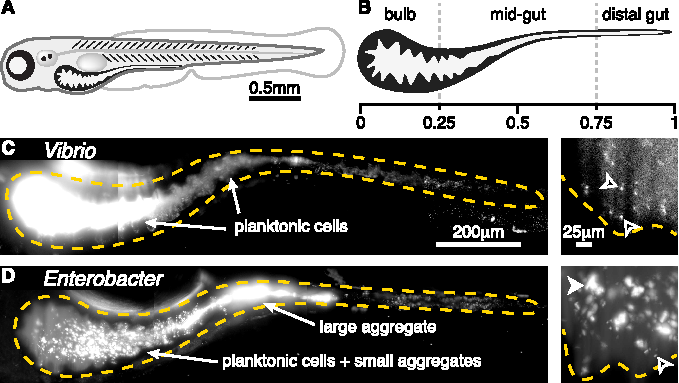
\includegraphics[width =4.75 in]{abx/fig1-eps-converted-to.pdf}}
	\caption{\textbf{Two bacterial species show different extremes of in vivo aggregation phenotypes.}  A: Schematic of a zebrafish 5 days post-fertilization (dpf). B: Schematic of the larval zebrafish intestine with numbers denoting approximate fraction of gut length. C: \textit{Vibrio cholerae} ZWU0020 in vivo. Left: a maximum intensity projection of a three-dimensional image of the full gut. Dense, bright bacteria and dimmer intestinal autofluorescence are evident. The orange dashed curve indicates a coarse outline of the gut boundary. Scale bar: 200 $\mu$m. Right: a single optical plane within the anterior bulb in a fish colonized with 1:100 green fluorescent protein (GFP): dTomato (dTom)-expressing \textit{Vibrio}, with the GFP channel shown to highlight individual microbes in the dense swarm. The orange dashed curve indicates the approximate contour of the intestinal epithelium. Black arrowheads indicate examples of single planktonic cells. Scale bar: 25 $\mu$m. (See also SI Movie 1) D: \textit{Enterobacter cloacae} ZOR0014 in vivo, shown as a maximum intensity projection of the full gut (left) and a subset of the same projection in the anterior bulb (right); bacterial aggregates are evident. The black arrowhead indicates an example of a single planktonic cell; the white arrowhead indicates an example of a multicellular aggregate. Scale bars same as in (C).}
\end{figure*}


Conventional wisdom regarding bacterial responses to antibiotic drugs, derived largely from in vitro assays, holds that drug tolerance is facilitated by low growth rates and biofilm formation \cite{walters2003contributions,fux2005survival}. Recent work suggests that microbes in the vertebrate gastrointestinal tract adopt a variety of growth and aggregation phenotypes \cite{korem2015growth,schlomann2018bacterial,Moor2017,welch2017spatial}, raising the question of whether antibiotic susceptibility in the gut bears the same relationship to kinetics and physical structure as in less dynamic environments, or whether the strong mechanical activity and large fluid flows present in the intestine \cite{cremer2017effect} lead to fundamentally different rules.

To investigate the in vivo response of gut bacteria to low-dose antibiotic exposure, especially the relationship between susceptibility and bacterial behavior, we conducted live imaging-based studies of larval zebrafish (Fig. 1A, 1B), spanning the entire intestinal volume with spatial and temporal resolutions not attainable in humans or other model vertebrates. We focused our study on two native zebrafish bacterial isolates, both frequently found in the intestine \cite{Stephens2016}, that we identified as representing extremes of growth and aggregation phenotypes \cite{schlomann2018bacterial}. The first, \textit{Vibrio cholerae} ZWU0020, hereafter referred to as ``\textit{Vibrio}'', exists in the larval zebrafish intestine primarily as dense populations of highly motile and planktonic individuals (Fig. 1C, SI Movie 1).  \textit{Vibrio} grows rapidly, with an in vivo doubling time of approximately 1 hour (exponential growth rate of 0.8 $\pm$ 0.3 1/hr) \cite{Wiles2016}. The second,  \textit{Enterobacter cloacae} ZOR0014, hereafter referred to as ``\textit{Enterobacter}'' primarily forms large, dense bacterial aggregates with small sub-populations of non-motile planktonic cells (Fig. 1D, SI Movie 2) \cite{Wiles2018} and has an in vivo doubling time of approximately 2.5 hours (exponential growth rate of 0.27 $\pm$ 0.05 1/hr) (SI Appendix, Fig. S1). To delineate and quantify antibiotic responses independent of inter-bacterial competition, we studied \textit{Vibrio} and \textit{Enterobacter} separately in hosts that were initially raised germ-free (Materials and Methods). We assessed response dynamics of each bacterial population after treatment with the antibiotic ciprofloxacin, a broad spectrum fluoroquinolone that interferes with DNA replication by inhibiting DNA gyrase. Ciprofloxacin is widely administered therapeutically and has been used as a model antibiotic in studies of human microbiome disruption  \cite{relmanABX_2011}. Furthermore, ciprofloxacin is often detected in environmental samples at ng/ml concentrations that are sublethal but capable of perturbing bacterial physiology \cite{girardi2011biodegradation, goneau2015subinhibitory}. 


As detailed below, we discovered that sublethal levels of ciprofloxacin lead to major reductions in intestinal abundance of both \textit{Vibrio} and \textit{Enterobacter} that could not be predicted from in vitro responses alone. In contrast to conventional wisdom, the slow-growing and highly aggregated \textit{Enterobacter} was impacted far more severely than the fast-growing, planktonic \textit{Vibrio}. Changes in bacterial abundances were driven primarily by clearance from the intestine by peristaltic-like fluid flow, which impacts aggregated bacteria more severely than planktonic cells. Exposure to sublethal levels of ciprofloxacin shifted both species to a more aggregated state, but for \textit{Enterobacter} this state was unsustainable and led to population collapse and extinction. Quantitative image-derived population data motivate and are well fit by physical models originally used to describe colloidal growth and polymer gelation, implying an antibiotic-induced phase transition in bacterial community physical structure and revealing a general framework for understanding and predicting intestinal antibiotic perturbations.






\begin{figure*}[h]
\centerline{
	%\includegraphics[width =4.75 in]{abx/fig2.eps}}
	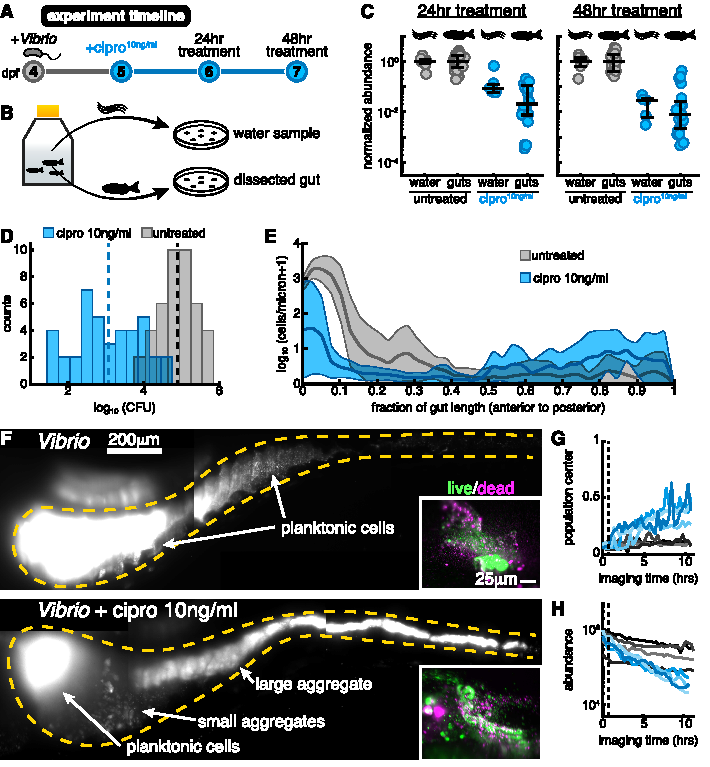
\includegraphics[width =4.75 in]{abx/fig2-eps-converted-to.pdf}}
	\caption{\textbf{Low-dose ciprofloxacin induces \textit{Vibrio} aggregation and expulsion in vivo.} A: Schematic of the experimental timeline. B: Schematic of the sampling scheme for plating measurements. C: Normalized abundances (number of colony forming units (CFUs) scaled by untreated medians) of water and gut populations. $N$ values left to right: 8, 24, 7, 20, 6, 18, 5, 20. Water $N$ values denote number of flasks; gut $N$ values denote number of fish. D: Histograms of gut CFUs with pooled data from 24 and 48 h treatments. Counts indicate the number of individual fish with a given log$_{10}$ \textit{Vibrio} CFUs. Dashed lines indicate the mean of each set, showing a $\sim$100-fold reduction in intestinal \textit{Vibrio} abundance in antibiotic-treated fish. E: Ensemble-averaged spatial distributions of log-transformed cell density as a function of distance along the gut axis, integrated over the perpendicular dimensions. F: Maximum intensity projections of 3D images of untreated (top) and ciprofloxacin-treated (bottom) \textit{Vibrio} populations. Insets: Viability staining of bacteria expelled from the gut, with green and magenta indicating living and dead cells, respectively. G-H: Dynamics of in vivo \textit{Vibrio} populations untreated (grey lines) and treated with 10 ng/ml ciprofloxacin (blue lines). G: 1D center of mass, normalized to intestine length. H: Total image-derived \textit{Vibrio} abundance. In both (G) and (H), each curve represents a different zebrafish. Vertical dotted lines indicate the time of drug administration to the treatment cohort, $t = 0.67$ hours.}
\end{figure*}


\section*{Results}

\subsection*{Low-dose ciprofloxacin increases bacterial aggregation and intestinal expulsion}

For both \textit{Vibrio} and \textit{Enterobacter}, we empirically determined a ciprofloxacin dosage that induced clear changes in bacterial physiology and behavior in vitro, but that was below the apparent minimum inhibitory concentration. We first describe results of antibiotic exposure, in vitro and in vivo, for the \textit{Vibrio} species. 

From an initial survey of dose-response in rich media, we identified 10 ng/mL ciprofloxacin as an appropriate exposure for \textit{Vibrio} populations. Growth of \textit{Vibrio} in lysogeny broth in the presence of 1 ng/ml ciprofloxacin closely resembles that of the untreated control, while a concentration of 100 ng/ml is largely inhibitory (SI Appendix, Fig. S2A). An intermediate concentration of 10 ng/ml leads to a stable, intermediate optical density. Viability staining (Materials and Methods) after 6 hours of incubation with 10 ng/ml ciprofloxacin identifies 30-80\% of cells as alive (SI Appendix, Fig. S3A and S3B), again consistent with this antibiotic concentration being sufficient to perturb the bacterial population without overwhelming lethality. Growth in the presence of 10 ng/ml ciprofloxacin induces marked changes in cell morphology and motility: treated cells exhibit filamentation, making them considerably longer (mean $\pm$ std. dev. 5.3 $\pm$ 3.1 $\mu$m) than untreated \textit{Vibrio} (2.9 $\pm$ 0.9 $\mu$m) (SI Appendix, Fig. S2B). Swimming speed was also reduced compared to untreated cells (mean $\pm$ std. dev. 11.4 $\pm$ 7.2 $\mu$m/s, untreated  16.9 $\pm$ 11.1 $\mu$m/s) (SI Appendix, Fig. S2C, SI Movies 3 and 4). We note also that 10 ng/ml ciprofloxacin is comparable to levels commonly measured in environmental samples \cite{girardi2011biodegradation}. 

While useful for illuminating the appropriate sub-lethal concentration to further examine, experiments in rich media conditions are not an optimal assay for comparison of in vitro and in vivo antibiotic treatments, as the chemical environments are likely very dissimilar. We therefore assessed effects of ciprofloxacin on bacterial populations in the aqueous environments of the flasks housing the larval zebrafish in comparison to populations in the intestines. In the flask water, as in the intestine, the only nutrients are fish-derived. Oxygen levels are  comparable to those in the larval gut, due to fast diffusion and the animals' small size. Bacteria in flask water therefore constitute a useful baseline against which to compare antibiotic impacts on intestinal populations.

\textit{Vibrio} was associated with germ-free zebrafish at 4 days post-fertilization (dpf) by inoculation of the aqueous environment at a density of 10$^6$ cells/ml (Materials and Methods) and allowed to colonize for 24 hours, which based on previous studies provides ample time for the bacterial population to reach its carrying capacity of approximately $10^5$ cells/gut \cite{Wiles2016}. Animals and their resident \textit{Vibrio} populations were then immersed in 10 ng/ml ciprofloxacin for 24 or 48 hours, or left untreated (Fig. 2A and 2B). \textit{Vibrio} abundances in the gut were assayed by gut dissection and plating to measure colony forming units (CFUs) (Materials and Methods). Abundances in the flask water were similarly assayed by plating. We quantified the effect of the antibiotic treatment by computing the ratio of bacterial abundances in the treated and untreated cases, resulting in a normalized abundance (Fig. 2C). After a 24 hour treatment, log$_{10}$-transformed abundances in the flask water dropped by $0.98 \pm 0.4$ (mean $\pm$ std. dev.) compared to untreated controls, or one order of magnitude on average. In contrast, log$_{10}$-transformed intestinal abundances showed a more severe reduction of $1.75 \pm 0.88$ (Fig. 2C), or a factor of approximately 60 on average, suggesting that the intestinal environment amplifies the severity of ciprofloxacin treatment. For the 48 hour treatment, the declines in flask water and intestinal abundances were similarly severe (Fig. 2C). In terms of absolute abundances, pooled data from 24 and 48 hour treatments gives a mean $\pm$ std. dev. of the log$_{10}$-transformed \textit{Vibrio} population of 3.1 $\pm$ 0.9 ($n = 40$), compared to 4.9 $\pm$ 0.5 ($n = 42$) for untreated specimens (Fig. 2D). Unpooled data are similar (SI Appendix, Fig. S3E, S3F).  


To assess the possibility that the intestine makes \textit{Vibrio} more susceptible to ciprofloxacin-induced cell death, we embedded larval zebrafish in a 0.5\% agarose gel, which allowed collection of expelled bacteria. After staining expelled bacterial cells with the viability dyes SYTO9 and propidium iodide, we imaged ejected material. We found  no detectable difference between ciprofloxacin-treated and untreated populations (Fig. 2F, insets). Similarly sizeable fractions of viable and non-viable cells are evident in both ciprofloxacin-treated and untreated populations; however, co-staining of zebrafish host cells hindered exact quantification (SI Appendix, Fig. S4). This result suggests that the ciprofloxacin-induced population decline observed in vivo occurs independent of overt cell death and is a consequence of the response of living bacteria to the intestinal environment. We further note that the dose-response of the intestinal \textit{Vibrio} abundance (SI Appendix, Fig. S5) mirrors the dose-response of the in vitro growth rate, implying that the larval gut does not significantly alter or concentrate ciprofloxacin. This is also consistent with the widespread use of zebrafish larvae as a  pharmacological screening platform, as water soluble chemicals readily enter and leave the animal \cite{rennekamp201515,yoganantharjah2017use}.

To investigate the causes of ciprofloxacin's disproportionately large impact on in vivo bacterial abundance, we used light sheet fluorescence microscopy to directly monitor \textit{Vibrio} populations within the intestine over several hours as they responded to antibiotic exposure. Three-dimensional time-lapse imaging revealed that within hours of ciprofloxacin treatment, large numbers of bacteria became depleted from the anterior-localized planktonic and motile population (SI Movies 5 and 10). Cells were instead found in the mid and distal regions of the gut, where they appeared to be condensed into large multicellular aggregates prior to being expelled from the gut altogether (SI Movies 5 and 11). After 10 hours of exposure, \textit{Vibrio} populations in ciprofloxacin-treated hosts contained large, 3D aggregates localized to the posterior of the intestine, a feature not observed in untreated controls (Fig. 2E and 2F) nor in all previous characterizations of this strain \cite{Wiles2016,schlomann2018bacterial}. We note also that in vitro, antibiotic-treated \textit{Vibrio} does not form large aggregates (SI Appendix, Fig. S3 and S6, SI Movie 4)

To determine whether the bacterial aggregation observed in vivo stems from a fundamentally different response to antibiotics at the single-cell level or different large-scale consequences of similar cell-level response, we generated in \textit{Vibrio} a genetically encoded fluorescent reporter of the SOS pathway (SI Appendix, Fig. S7, Materials and Methods), a DNA damage repair pathway induced by genotoxic agents such as ciprofloxacin \cite{erill2007aeons,kreuzer2013dna}. Genes in the SOS regulon halt replication and enable DNA repair, and also affect motility and biofilm formation \cite{irazoki2016sos,goneau2015subinhibitory}. In vitro, we found that treatment with 10 ng/ml ciprofloxacin strongly induced \textit{recN}-based SOS reporter activity, with a heterogeneous response across individual cells (SI Appendix, Fig. S3C and S3D). Within the intestine, SOS reporter activity was also heterogeneous, appearing in both planktonic and aggregated cells. Planktonic cells that were SOS-positive appeared more filamented and less motile compared to SOS-negative cells within the same host (SI Movie 6). The activation of the SOS reporter in vitro and in vivo by ciprofloxacin (SI Movie 6 and Fig S3C and S3D) suggests that in both cases a canonical SOS response is involved in the perturbation of \textit{Vibrio} physiology. 

Together, these data begin to reveal a mechanism by which the intestine amplifies the effect of low-dose ciprofloxacin. Individual \textit{Vibrio} cells first undergo an SOS response that is associated with changes in cellular morphology and behavior. In the context of the mechanical activity of the intestine, these molecular and cellular-level changes then give rise to population-level aggregation and spatial reorganization throughout the entire length of the intestine, with the population shifting its center of mass posteriorly (Fig. 2G, $n=4$ per case). This process culminates in the expulsion of large bacterial aggregates from the host, causing a precipitous decline in total bacterial abundance (Fig. 2H).

\begin{figure*}[h]
\centerline{
	%\includegraphics[width =4.75 in]{abx/fig3.eps}}
	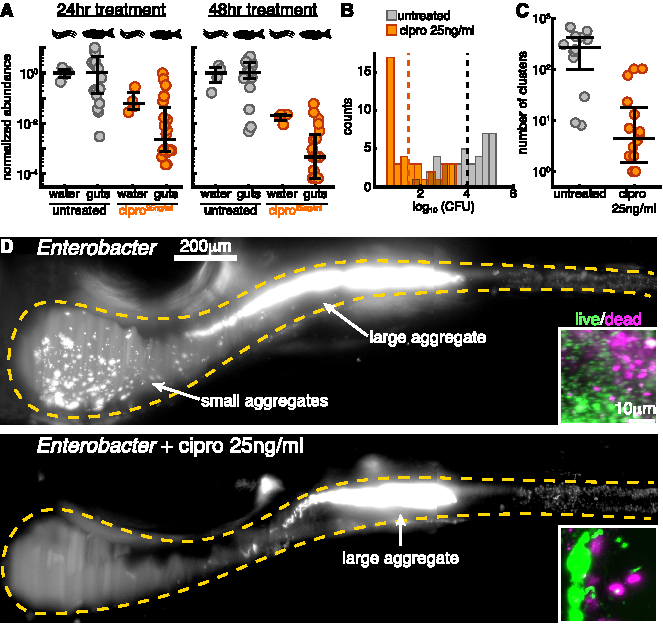
\includegraphics[width =4.75 in]{abx/fig3-eps-converted-to.pdf}}
	\caption{\textbf{Low-dose ciprofloxacin collapses \textit{Enterobacter} populations and suppresses small clusters in vivo.} A: Normalized abundances (number of colony forming units (CFUs) scaled by untreated medians) of water and gut populations. $N$ values left to right: 4, 20, 4, 20, 4, 19, 4, 20. Water $N$ values denote number of flasks; gut $N$ values denote number of fish. B: Histograms of gut CFUs with pooled data from 24 and 48 h treatments. Counts indicate the number of individual fish with a given log$_{10}$ \textit{Enterobacter} CFUs. Dashed lines indicate the mean of each set, showing a $\sim$1000-fold reduction in intestinal \textit{Enterobacter} abundance in antibiotic-treated fish. C: Total number of bacterial clusters in the intestine, quantified from 3D images (Materials and Methods). D: Maximum intensity projections of 3D images of untreated (top) and ciprofloxacin-treated (bottom) \textit{Enterobacter} populations. Insets: Viability staining of bacteria expelled from the gut, with green and magenta indicating living and dead cells, respectively.}
\end{figure*}


\subsection*{Low-dose ciprofloxacin suppresses small cluster reservoirs associated with intestinal persistence}

In contrast to \textit{Vibrio}, \textit{Enterobacter} is slower growing, non-motile, and naturally forms dense aggregates within the zebrafish intestine. \textit{Enterobacter} populations have an in vivo growth rate of 0.27 $\pm$ 0.05 h$^{-1}$ (mean $\pm$ std. dev, SI Appendix, Fig. S1), compared to 0.8 $\pm$ 0.3 h$^{-1}$ for \textit{Vibrio} \cite{Wiles2016}. Based on conventional notions of antibiotic tolerance, we hypothesized that \textit{Enterobacter} would be less affected by ciprofloxacin treatment than the fast growing, planktonic \textit{Vibrio}. However, as detailed below, we found this prediction to be incorrect; \textit{Enterobacter} exhibits an even greater response  to low-dose ciprofloxacin.

We first established in vitro that 25 ng/ml ciprofloxacin produces similar effects on \textit{Enterobacter} growth as did 10 ng/ml exposure on \textit{Vibrio}. With the identical inoculation procedure used for \textit{Vibrio}, log$_{10}$-transformed \textit{Enterobacter} abundance in the flask water dropped by 1.2 $\pm$ 0.4 (mean $\pm$ std. dev.) compared to untreated controls after 24 hours, and dropped by $1.8 \pm 0.2$ after 48 hours (Fig. 3A). These values match well the values for \textit{Vibrio}: 0.98 $\pm$ 0.37 for 24 hours, 1.81 $\pm$ 0.5 for 48 hours. Assays in rich media show a similarly reduced density between the two species (SI Appendix, Fig. S8) and an even lesser degree of cell death and damage in vitro for  \textit{Enterobacter} as compared to \textit{Vibrio}, with a viable fraction of approximately 95\% (SI Appendix, Fig. S9A and S9B). As with \textit{Vibrio}, in vitro growth measurements and viability staining both imply that low-dose ciprofloxacin treatment of \textit{Enterobacter} induces growth arrest rather than widespread lethality.

Strikingly, low-dose ciprofloxacin treatment of fish colonized with \textit{Enterobacter}  (Materials and Methods) resulted in even greater reductions in abundance than in the case of \textit{Vibrio}, with the majority of populations becoming nearly or completely extinct during the assay period (Fig. 3A and 3B). Inoculation, treatment, dissection, and plating were performed as for \textit{Vibrio} (Materials and Methods). Compared to untreated controls, log$_{10}$-transformed intestinal abundances were reduced by 2.3 $\pm$ 1.1 after 24 hours, and by 3.2 $\pm$ 1.0 after 48 hours (Fig. 3A). These reductions in intestinal abundances greatly exceeded the reductions of bacterial abundances in the flask water (Fig 3A). In terms of absolute abundances, pooled data from 24 and 48 hour treatments gives a mean $\pm$ std. dev. of the log$_{10}$-transformed \textit{Enterobacter}  population of 1.5 $\pm$ 1.0 ($n=40$), compared to 4.0 $\pm$ 1.0 ($n=39$) for untreated specimens (Fig. 3B); unpooled data are similar (SI Appendix, Fig. S9C and S9D). 

Live imaging of intestinal populations at single time points revealed approximately 40\% of treated hosts to be devoid or nearly devoid of \textit{Enterobacter}, consistent with the plating-based measurements. In hosts that contained appreciable bacterial populations we observed a clear difference between treated and untreated specimens: \textit{Enterobacter}  populations in ciprofloxacin-treated hosts contained fewer small bacterial clusters and fewer individual planktonic cells than untreated controls (Fig. 3C and 3D). We quantified this distinction using computational image analysis to identify each cluster (Materials and Methods), defining a single cell as a cluster of size one. Bacterial populations in ciprofloxacin-treated animals contained $\sim$80x fewer clusters than untreated animals (Fig. 3C). Viability staining showed that there were no obvious differences in the viable fractions of bacteria expelled from the intestines of untreated and treated hosts (Fig. 3D, insets, SI Appendix, Fig. S10). As with \textit{Vibrio}, these observations suggested that the reduction in \textit{Enterobacter}'s intestinal abundance was independent of cell death.  


Previous studies of other naturally aggregated bacterial species have revealed that large bacterial aggregates are highly susceptible to expulsion from the gut \cite{Wiles2016,Logan2018}. To establish whether this is also the case for \textit{Enterobacter} in the absence of low-dose ciprofloxacin treatment, we performed time-lapse 3D imaging (Materials and Methods). Indeed, in 2 out of 5 hosts imaged for 3.5 hours each, we observed events in which the largest bacterial aggregate was abruptly expelled from the intestine (Fig. 4A and SI Movie 7). These time-lapse movies also showed clear examples of cluster aggregation (SI Movie 8), in which single cells and small aggregates appear to come together and fuse, a process that is likely due to the rhythmic intestinal contractions that occur between frames. Importantly, smaller aggregates and planktonic cells that preferentially localize to the intestinal bulb are relatively undisturbed during these expulsion events, save for a few clusters that become incorporated into the large mass during its transit (SI Movie 7). 

Our observations suggest an explanation of how low-dose ciprofloxacin can lead to dramatic drops in \textit{Enterobacter} abundance that moreover illuminates the more general question of how naturally aggregating bacterial species can persist in the vertebrate gut in spite of transport-driven expulsion. We provide both a qualitative and a quantitative description of the relevant dynamics, beginning with the following conceptual model: single cells of \textit{Enterobacter}  replicate to form small clusters, which then aggregate to form larger clusters under the influence of intestinal flow. Large clusters are transported by the rhythmic contractions of the gut \cite{Wiles2016,Logan2018,ganz2018} and are stochastically expelled from the host \cite{Wiles2016,Logan2018}. The individual bacteria and small clusters that remain within the intestine serve as a reservoir that reseeds the next population, and the process of replication, aggregation, and expulsion repeats. Therefore, persistence  within the intestine requires processes that generate single cells or small clusters, otherwise transport will eventually lead to extinction. This reseeding could take the form of (i) immigration of new cells from the environment, (ii) passive fragmentation of  clusters, or (iii) active fragmentation in which single cells break away from a cluster surface during cell division. Immigration from the environment likely occurs even in established populations, but measurements in larval zebrafish suggest very low rates of immigration \cite{robinson2018experimental}. We therefore suspected that more robust mechanisms must promote persistence. Supporting the active fragmentation mechanism, we found in untreated hosts examples of \textit{Enterobacter} populations that contain an abundance of single cells, a single large aggregate, and a lack of mid-sized aggregates (SI Appendix, Fig. S9E). Following low-dose ciprofloxacin treatment, the planktonic cell reservoir associated with resilience to intestinal transport is depleted (Fig. 3C), most likely due to stalled \textit{Enterobacter} division (SI Appendix, Fig. S8), leading to collapse of the resident bacterial population (Fig. 3A and 3B).




\subsection*{A quantitative model of bacterial cluster dynamics}

\begin{figure*}[h]
\centerline{
	%\includegraphics[width =4.75 in]{abx/fig4.eps}}
	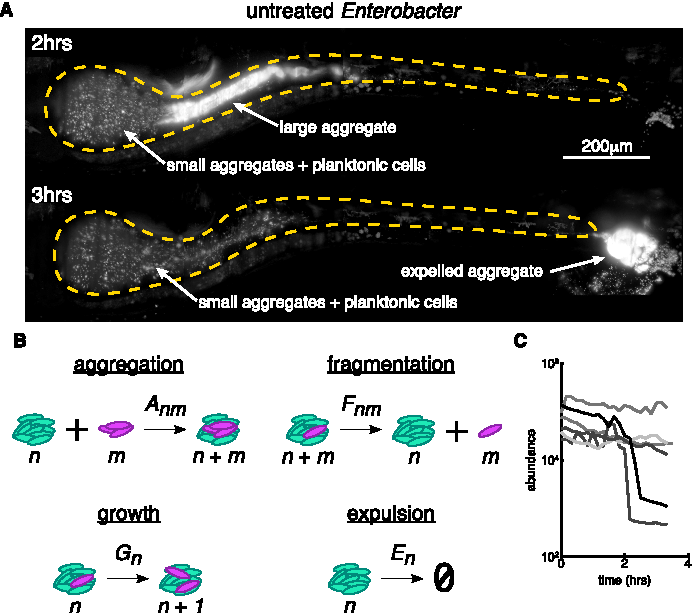
\includegraphics[width =4.75 in]{abx/fig4-eps-converted-to.pdf}}
	\caption{\textbf{Small bacterial clusters are required for recovery after large expulsion events.}  A: Maximum intensity projections of untreated \textit{Enterobacter} populations before (top, $t=2$ hours from the start of imaging) and after (bottom, $t=3$ hours) an expulsion event (See also SI Movie 5). Scale bar = 200 $\mu$m. B: Schematic of a kinetic model of bacterial cluster dynamics, illustrating its four constituent processes. C: Image-derived time-series of \textit{Enterobacter} abundance in five untreated hosts showing sporadic large expulsion events.}
\end{figure*}

To solidify and test our conceptual picture, we developed a predictive mathematical model of bacterial cluster dynamics. We describe the framework of the model, its validation, and general insights it provides into perturbations and population stability. Drawing on ideas from non-equilibrium statistical mechanics and soft matter physics, we constructed a general kinetic model that describes the time evolution of a collection of bacterial clusters with varying sizes, illustrated schematically in Fig. 4B. We posit that four processes govern cluster dynamics: aggregation, fragmentation, growth, and expulsion.  Each is described by a kernel that specifies its rate and size dependence: (1) aggregation of a cluster of size $n$ and a cluster of size $m$ occurs with rate $A_{nm}$; (2) fragmentation of a cluster of size $n+m$ into clusters of size $n$ and $m$ occurs with rate $F_{nm}$; (3) growth (due to cell division) of a cluster of size $n$ occurs with rate $G_n$; (4) expulsion (removal by intestinal transport) of a cluster of size $n$ occurs with rate $E_n$. Note that condensation of the population into a single massive cluster poises the system for extinction, for any nonzero $E_n$. The model is non-spatial and is inspired by well established frameworks for nucleation and growth phenomena such as polymer gelation and colloidal aggregation \cite{krapivsky2010kinetic}. For example, sol-gel models describe a transition between dispersed individual units (``sol") and a system-spanning connected network (``gel") in materials capable of polymerization. In the thermodynamic limit of infinite system size, the model  can be studied using standard analytic techniques \cite{krapivsky2010kinetic}. However, unlike polymer solutions and other bulk systems for which the possible number of clusters is effectively unbounded, our intestinal populations are constrained to have at most a few hundred clusters (Fig. 3C), necessitating the use of stochastic simulations (Materials and Methods).

In its general form, the model encompasses a wide range of behaviors that can be encoded in the various functional forms possible for the rate kernels $A_{nm}$ $F_{nm}$, $G_n$, and $E_n$. Based on our observations and theoretical considerations elaborated in the Materials and Methods section, we made the following assumptions: (1) the rate of aggregation between two clusters is independent of their size, $A_{nm} = \alpha$;  (2) fragmentation occurs only by separation of single cells and with a rate that is independent of cluster size, $F_{nm} = \beta$ for $m=1$ and $F_{nm}=0$ otherwise; (3) growth is logistic with a global carrying capacity, $G_n = rn(1-N/K)$ with $N$ the total number of cells, $r$ the per capita growth rate, and $K$, the carrying capacity; (4) expulsion is independent of cluster size, $E_n = \lambda$.  This model contains as special cases various simple models of linear polymers \cite{krapivsky1996transitional} and also resembles recent work modelling chains of \textit{Salmonella typhimurium} cells in the mouse gut \cite{bansept2019enchained}.  As discussed in the SI Appendix, these choices constitute the minimal model consistent with theoretical constraints and experimental phenomenology. More complex models are of course possible, but the requisite increase in the number of adjustable parameters would result in a trivial but meaningless ability to fit the observed data.
  

Even with the assumptions described above, the model needs 5 parameters: rates of aggregation, fragmentation, growth, and dispersal, and a global carrying capacity. However, all of these parameters can be set by experimentally derived values unrelated to cluster size distributions. We measured \textit{Enterobacter}'s per capita growth rate by performing time-lapse imaging of initially germ-free hosts that had been exposed to \textit{Enterobacter} for only 8 hours, capturing the exponential increase of a small founding population (SI Appendix, Fig. S1, SI Movie 9), yielding $r = 0.27 \pm 0.05$ hr$^{-1}$ (mean $\pm$ std. dev across $n=3$ hosts). We identified expulsion events as abrupt collapses in \textit{Enterobacter} abundance from time-lapse images (Fig. 3C, SI Movie 7) and set the expulsion rate equal to the measured collapse rate, $\lambda = 0.11 \pm 0.08$ hr$^{-1}$ (mean $\pm$ standard error, assuming an underlying Poisson process (Materials and Methods)). The model can be simulated to provide the mean and variance of the $\log_{10}$-transformed abundance distribution at a given time for a given set of parameters. Using this approach, we fit static bacterial abundance measurements from dissection and plating at 72 hours post-inoculation (Materials and Methods) to determine the carrying capacity, $K$, and the ratio of fragmentation and aggregation rates, $\beta/\alpha$. As discussed in the Materials and Methods section, the cluster dynamics should depend primarily on the ratio of $\beta/\alpha$ rather than either rate separately. This yielded $\log_{10}K = 5.0 \pm 0.5$ and $\log_{10}\beta/\alpha =  2.5 \pm 0.4$.


The model therefore allows a parameter-free prediction of the size distribution of \textit{Enterobacter} aggregates, plotted in Fig. 5A together with the measured distribution derived from three-dimensional images, averaged across 12 untreated hosts. The two are in remarkable agreement. We also plot, equivalently, the cumulative distribution function $P(\text{size} > n)$, the probability that a cluster will contain greater than $n$ cells, again illustrating the close correspondence between the data and the prediction and validating the model. We emphasize that no information about the cluster size distribution was used to estimate any of the model parameters. We further note that the cluster size distribution is a stringent test of the model's validity. Other cluster models predict different forms, typically with steep tails \cite{krapivsky1996transitional,bansept2019enchained}. The linear chain model of \cite{bansept2019enchained}, for example, leads to an exponential distribution of cluster sizes that does not match the shallower, roughly power-law form of our data.


\begin{figure*}%[h]
\centerline{
	%\includegraphics[width =4.75 in]{abx/fig5.eps}}
	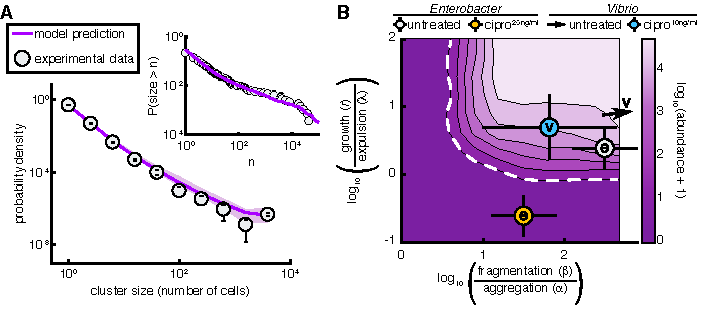
\includegraphics[width =4.75 in]{abx/fig5-eps-converted-to.pdf}}
	\caption{\textbf{A stochastic kinetic model predicts bacterial cluster sizes and generates a phase diagram for in vivo abundance.}  A: The distribution of image-derived \textit{Enterobacter} cluster sizes (grey circles) along with the prediction of our stochastic model (purple line). There are no free parameters in the fit; values were fixed by abundance, growth, and expulsion rate measurements independent of cluster size. Parameters: $r = 0.27$ hr$^{-1}$, $\lambda = 0.11$ hr$^{-1}$, $\alpha = 0.1$ hr$^{-1}$, $\beta = 10^{1.5}$ hr$^{-1}$, $K = 10^5$. Error bars on experimental data are standard deviations across hosts. Shaded confidence intervals for the model prediction are bounds from parameter uncertainties. Inset: The same experimental data and model plotted without binning as a reverse cumulative distribution. B: Phase diagram of the log-transformed abundance, $\langle \log_{10}(N+1)\rangle$, showing the extinction transition (white dashed line). From best fit parameter estimates, the in vivo state of untreated \textit{Enterobacter} is overlaid as a grey circle, and 25 ng/ml ciprofloxacin-treated \textit{Enterobacter} as an orange circle; both circles are marked with ``e''. Untreated \textit{Vibrio} is located off the scale, indicated by the arrow, 10 ng/ml ciprofloxacin treated \textit{Vibrio} is overlaid as a cyan circle marked with ``v''. The doses for \textit{Enterobacter} and \textit{Vibrio} were established to be approximately equivalent in vitro. Parameters: $\lambda = 0.11$ hr$^{-1}$, $\alpha =  0.1$ hr$^{-1}$, $K = 10^5$ were fixed; $r$ and $\beta$ were varied on logarithmic grids.}
\end{figure*}



\subsection*{The abundance phase diagram and extinction transition}

Our kinetic model provides insights into the consequences of low-dose antibiotic perturbations on gut bacterial populations. We consider a general phase diagram of possible growth, fragmentation, aggregation, and expulsion rates, and then situate \textit{Enterobacter} in this space. For simplicity of illustration, we consider a two-dimensional representation with one axis being the ratio of the fragmentation and aggregation rates, $\beta/\alpha$, and the other being the ratio of the growth and expulsion rates, $r/\lambda$ (Fig. 5B). As noted above and in the Materials and Methods section, the model in the regime studied should depend on the ratio $\beta/\alpha$ rather than on $\beta$ or $\alpha$ independently. However, the roles of $r$ and $\lambda$ are not simply captured by their ratio. The expulsion rate nonetheless provides a scale to which to compare the growth rate, $r$, and we plot Fig. 5B using  $r/\lambda$  calculated for fixed $\lambda = 0.11$ hr$^{-1}$, the measured value. For completeness, we show a three-dimensional $r,  \lambda, \beta/\alpha$ phase diagram as SI Appendix, Figure S11E and S11F. We numerically calculated the steady state phase diagram of the model (Materials and Methods) and show in Figure 5B the mean log-transformed abundance, $\langle\log_{10}(N+1)\rangle$. The regime of extinction $(N=0)$ is evident (dark purple, with dashed white boundary ). 


The data-derived parameter values place untreated intestinal \textit{Enterobacter} fairly close to the extinction transition (Fig. 5B). An antibiotic-induced growth rate reduction of approximately 5x is sufficient to cross the boundary to the $N=0$ regime (i.e. to extinction), moving downward in Fig. 5B. This growth rate reduction, or an equivalent increase in death rate, reflects the conventional view of antibiotic effects.  An approximately 300x reduction in the balance between fragmentation and aggregation spurs an alternative path to extinction, moving leftward in Fig. 5B, reflecting a distinct mechanism resulting solely from changes in physical structure. The extinction transition in this direction corresponds to the condensation of the population into a single cluster, reminiscent of gelation phase transitions in polymer systems. As described above, low-dose ciprofloxacin causes a strong reduction in the number of small bacterial clusters, lowering $\beta$ and possibly also $r$ if fragmentation and individual cell division are linked. Conservatively assuming an equal effect along both axes, and fitting simulations to the 24 hour treatment abundances (Materials and Methods), we find that the antibiotic reduces $r$ and $\beta/\alpha$ by $\sim$10x. This drives the bacterial system through the phase boundary and well into the extinction regime (Fig. 5B, orange circle), consistent with our observations. 

In contrast to \textit{Enterobacter}, treatment of \textit{Vibrio} with ciprofloxacin does not lead to widespread extinction after 48 hours, suggesting that treated populations either lie safely at a new steady state away from the extinction boundary, or are close enough to the transition so that dynamics are slow. To estimate model parameters for ciprofloxacin-treated \textit{Vibrio}, we performed a two parameter fit of $(\beta/\alpha, r)$ to the 24 hour treatment abundances. Because of \textit{Vibrio}'s large population size ($\sim 10^5$ clusters), we modified the stochastic simulation procedure using a tau-leaping algorithm (Materials and Methods, SI Appendix, Fig. S12). We indeed find ciprofloxacin-treated \textit{Vibrio} is located close to but safely inside the extinction boundary (Fig. 5B). Untreated \textit{Vibrio} populations show no appreciable multicellular aggregation and are located off-scale far to the upper-right side of the phase diagram (Fig. 5B, arrow).  



\section*{Discussion}

We have discovered that sublethal levels of a commonly used antibiotic can reduce the intestinal abundance of bacterial populations much more severely than would be predicted from in vitro responses, and that this amplification is a consequence of drug-induced changes to the bacterial groups' spatial architecture. Contrary to conventional notions of antibiotic tolerance, largely derived from in vitro studies, reductions in bacterial abundances were greater for the slow-growing, aggregated \textit{Enterobacter} species than for the fast-growing, planktonic \textit{Vibrio}. Live imaging revealed drug-induced increases in bacterial cohesion that, coupled to gut mechanical activity, lead to the expulsion of viable bacterial cells. The microscopic details of this cohesion, likely involving cell wall characteristics, mechanical compression by the gut wall and fluid flows, and perhaps intestinal mucus rheology, remain to be explored.

Notably, the underlying processes of bacterial aggregation and host intestinal transport are found throughout the animal kingdom, suggesting a general relevance beyond zebrafish that may explain, for example, data on weak antibiotics having strong effects on mammalian microbiomes \cite{cho2012antibiotics,schulfer2019impact}. Of course, chemical perturbations in more anatomically complex animals or non-gnotobiotic animals that house hundreds of resident bacterial species will undoubtedly involve additional processes beyond those uncovered here. We note, however, that responses to intestinal flow will influence bacterial population dynamics regardless of ecological complexity, and that our choice of model bacterial species spans the extremes of highly planktonic and highly cohesive strains, further implying generality. In the larval zebrafish, enhanced bacterial susceptibility to transport leads to expulsion from the gut. In larger or more complex intestines this may take the form of displacement from one region to a more distal region, with a corresponding shift in local nutrients or competitors, in addition to expulsion from the gut altogether.

The concentrations of ciprofloxacin examined here are commonly found in environmental samples, indicating a potentially widespread perturbation of animal gut microbiota due to antibiotic contaminants. In addition, the expulsion of live, antibiotic-exposed bacteria from animal intestines through the aggregation-based processes described here suggests a potential mechanism for enhanced spread of antibiotic resistance. This possibility is bolstered by our observation that in addition to aggregation, ciprofloxacin-treated cells undergo an active SOS response, which has been shown to promote mutation and horizontal gene transfer \cite{baharoglu2011vibrio,guerin2009sos,beaber2004sos}. Together, these observations underscore recent concerns about the public health risk posed by antibiotic contaminants in the environment \cite{national2018environmental}.

Our biophysical model of aggregation, fragmentation, growth, and expulsion describes our data well and provides testable predictions. It is remarkable, given the chemical and morphological complexity of even the larval zebrafish gut, that such a minimal model can accurately predict emergent properties such as the size distribution of bacterial aggregates. That this works is an indication of the power of theories of soft condensed matter physics, whose generality may prove useful in understanding the gut microbiome. Furthermore, our model supplies a framework for a quantitative understanding of gut microbial homeostasis in general. Like recent work modelling antibody-mediated enchaining of \textit{Salmonella} cells in the mouse gut \cite{bansept2019enchained}, our model implies that the physical processes of bacterial cluster formation and fragmentation play central roles in large-scale microbiota stability. We suggest that our cluster-dynamics model, validated by quantitative agreement between  predictions and in vivo data (Fig. 5A), may prove useful in less tractable host species such as mice and humans. Without live imaging or non-invasive sampling, it is challenging to estimate kinetic properties of microbial populations, such as aggregation rates. However, advances in histological sample preparation \cite{tropini2017gut} can preserve bacterial aggregates and yield cluster size distributions; inverting our model, such distributions can reveal the underlying in vivo bacterial kinetics.

Regarding antibiotics, the main prediction of our model is that naturally aggregated, slow growing bacteria will be impacted more severely than fast growing, planktonic species by equivalent low-dose antibiotic perturbations. This is contrary to conventional wisdom that links bacterial tolerance to reduced growth and increased aggregation  \cite{walters2003contributions,fux2005survival}, which stems from studies of antibiotic exposure in static or well-mixed environments. We find that in the intestine, where bacteria can be removed through fluid flow, there exist critical values of aggregation, fragmentation, growth, and expulsion rates, beyond which sustainable colonization becomes impossible (Fig. 5B). Naturally aggregated and slow-growing species are situated closer to this extinction phase boundary and are therefore more easily driven to population collapse by low-dose antibiotic perturbations. Intriguingly, new meta-omics methods \cite{korem2015growth} can be used to estimate in vivo growth rates of mammalian gut microbes, which would be interesting to correlate with antibiotic responses. We note in addition that inter-bacterial competition in the gut can be influenced by clustering and susceptibility to intestinal transport \cite{Wiles2016, Logan2018}, suggesting that competition outcomes could be altered by antibiotic treatment if changes in aggregation properties are different for different species. A final prediction of our model is that intestinal transport, which has been linked to microbiota composition \cite{cremer2017effect}, will influence the effects of low-dose antibiotic perturbations on microbial community composition. Combining pharmacological manipulations of intestinal transport with antibiotic treatments may therefore lead to novel strategies for precision engineering of the gut microbiome. 


\section*{Materials and Methods}
\subsection*{Animal care}
All experiments with zebrafish were done in accordance with protocols approved by the University of Oregon Institutional Animal Care and Use Committee and following standard protocols \cite{Westerfield2007}. 

\subsection*{Gnotobiology}
Wild-type (AB$\times$TU strain) zebrafish were derived germfree (GF) and colonized with bacterial strains as previously described \cite{Melancon2017} with slight modifications elaborated in the SI Appendix. 

\subsection*{Bacterial strains and culture}
\textit{Vibrio cholerae} ZWU0020 and \textit{Enterobacter cloacae} ZOR0014 were originally isolated from the zebrafish intestine \cite{Stephens2016}. Fluorescently marked derivatives of each strain were previously generated by Tn\textit{7}-mediated insertion of a single constitutively expressed gene encoding dTomato \cite{Wiles2018}. We note that all plating- and imaging-based experiments performed in this study were done using fluorescently marked strains, which carry a gentamicin resistance cassette, with the exception of experiments in which fluorescent dyes were used to assess viability of cells. Archived stocks of bacteria were maintained in 25\% glycerol at -80$^{\circ}$C. Prior to experiments, bacteria were directly inoculated from frozen stocks into 5 ml LB media (10 g/L NaCl, 5 g/L yeast extract, 12 g/L tryptone, 1 g/L glucose) and grown for $\sim$16 hours (overnight) shaking at 30$^{\circ}$C.
%

\subsection*{Culture-based quantification of bacterial populations} 
Dissection of larval guts was done as described previously \cite{milligan2011study}, with slight modifications elaborated in the SI Appendix. To compare the effect of ciprofloxacin on populations in the intestine and in the flask water, we normalized treated abundances by the corresponding untreated median abundance (Fig. 2C and 3A). To account for variation in untreated bacterial dynamics between weekly batches of fish, we performed the normalization within each batch. Unnormalized data is available in the SI Dataset.
%
%
\subsection*{Light sheet fluorescence microscopy of live larval zebrafish}
Live imaging of larval zebrafish was performed using a custom-built light sheet fluorescence microscope previously described in detail \cite{Jemielita2014}, with slight modifications elaborated in the SI Appendix.

%
\subsubsection*{Viability staining of expelled aggregates:}  Germ-free larval zebrafish were colonized with wild type \textit{Vibrio} or \textit{Enterobacter} (without fluorescent markers) for 24 hours and then mounted into agarose plugs using small glass capillaries identically to the imaging procedure (above). Individual capillaries were suspended into isolated wells of a 24-well tissue culture plate filled with embryo media containing anesthetic or anesthetic + ciprofloxacin (10 ng/ml for \textit{Vibrio}, 25 ng/ml for \textit{Enterobacter}) and the larvae were extruded from the capillaries. Fish remained mounted for 24 hours, during which expelled bacteria remained caught in the agarose plug. After treatment, fish were pulled back into the capillaries and transferred to smaller wells of a 96 well plate containing embryo media, anesthetic, and the LIVE/DEAD BacLight Bacterial Viability stains SYTO9 and propridium iodide. Fish were stained according to kit instructions, with the exception of the incubation period being extended from 15 to 30 min to account for potential issues with the aggregate nature of the cells \cite{netuschil2014confusion}.  Following staining, fish were pulled again into the capillaries and transferred to the light sheet microscope for imaging. As shown in the SI Appendix, Figures S4 and S10, zebrafish cells stain in addition to bacterial cells, precluding accurate quantification of viable fractions.

\subsection*{Image analysis}

Bacteria were identified in three-dimensional light sheet fluorescence microscopy images using a custom MATLAB analysis pipeline previously described \cite{Jemielita2014,schlomann2018bacterial}, with minor changes elaborated in the SI Appendix.


\subsection*{Kinetic model and stochastic simulations}
Simulation details are provided in the SI Appendix. In brief, Gillespie's direct method \cite{gillespie1977exact} was used to simulate stochastic aggregation, fragmentation, and expulsion events, while growth was treated as deterministic. To simulate \textit{Vibrio} populations, direct stochastic simulation becomes intractable due to the large number of clusters ($\sim 10^5$ single cells). We therefore implemented a modified tau-leaping algorithm \cite{gillespie2001approximate} that facilitates large simulations. We opted for a straightforward fixed $\tau$ method and empirically determined an optimal value of $\tau = 0.001$ h (SI Appendix, Fig. S12A,B). All simulations were written in MATLAB and code is available at INSERT URL %\url{https://github.com/bschloma/gac}.






\section*{Acknowledgements}
We thank Rose Sockol and the University of Oregon Zebrafish Facility staff for fish husbandry. Research was supported by an award from the Kavli Microbiome Ideas Challenge, a project led by the American Society for Microbiology in partnership with the American Chemical Society and the American Physical Society and supported by The Kavli Foundation. Work was also supported by the National Science Foundation under Awards 1427957 (R.P.) and 0922951 (R.P.), the M.J. Murdock Charitable Trust, and the National Institutes of Health (http://www.nih.gov/), under Awards P50GM09891 and P01GM125576-01 to K.G. and R.P., F32AI112094 to T.J.W., and T32GM007759 to B.H.S. The content is solely the responsibility of the authors and does not represent the official views of the NSF, National Institutes of Health, or other funding agencies. This work benefited from access to the University of Oregon high performance computer, Talapas.




%\bibliography{/Users/brandonschlomann/Documents/Gutz/PaperWriting/abx/abx_refs.bib}{}
%\bibliographystyle{unsrt}
%\begin{thebibliography}{10}
%
%\bibitem{dethlefsen2011incomplete}
%Dethlefsen L, Relman DA (2011) Incomplete recovery and individualized responses
%  of the human distal gut microbiota to repeated antibiotic perturbation.
%\newblock {\em Proceedings of the National Academy of Sciences} 108(Supplement
%  1):4554--4561.
%
%\bibitem{cho2012antibiotics}
%Cho I, et~al. (2012) Antibiotics in early life alter the murine colonic
%  microbiome and adiposity.
%\newblock {\em Nature} 488(7413):621.
%
%\bibitem{schulfer2019impact}
%Schulfer AF, et~al. (2019, doi:10.1038/s41396-019-0349-4, published online
%  ahead of print) The impact of early-life sub-therapeutic antibiotic treatment
%  ({STAT}) on excessive weight is robust despite transfer of intestinal
%  microbes.
%\newblock {\em The ISME Journal}.
%
%\bibitem{gaulke2016triclosan}
%Gaulke CA, Barton CL, Proffitt S, Tanguay RL, Sharpton TJ (2016) Triclosan
%  exposure is associated with rapid restructuring of the microbiome in adult
%  zebrafish.
%\newblock {\em PLoS One} 11(5):e0154632.
%
%\bibitem{andersson2014microbiological}
%Andersson DI, Hughes D (2014) Microbiological effects of sublethal levels of
%  antibiotics.
%\newblock {\em Nature Reviews Microbiology} 12(7):465.
%
%\bibitem{national2018environmental}
%"National Academies~of Sciences E, Medicine, others" (2018) {\em Environmental
%  Chemicals, the Human Microbiome, and Health Risk: A Research Strategy}.
%\newblock (National Academies Press).
%
%\bibitem{walters2003contributions}
%Walters MC, Roe F, Bugnicourt A, Franklin MJ, Stewart PS (2003) Contributions
%  of antibiotic penetration, oxygen limitation, and low metabolic activity to
%  tolerance of pseudomonas aeruginosa biofilms to ciprofloxacin and tobramycin.
%\newblock {\em Antimicrobial Agents and Chemotherapy} 47(1):317--323.
%
%\bibitem{fux2005survival}
%Fux C, Costerton JW, Stewart PS, Stoodley P (2005) Survival strategies of
%  infectious biofilms.
%\newblock {\em Trends in Microbiology} 13(1):34--40.
%
%\bibitem{korem2015growth}
%Korem T, et~al. (2015) Growth dynamics of gut microbiota in health and disease
%  inferred from single metagenomic samples.
%\newblock {\em Science} 349(6252):1101--1106.
%
%\bibitem{schlomann2018bacterial}
%Schlomann BH, Wiles TJ, Wall ES, Guillemin K, Parthasarathy R (2018) Bacterial
%  cohesion predicts spatial distribution in the larval zebrafish intestine.
%\newblock {\em Biophysical Journal} 115(11):2271--2277.
%
%\bibitem{Moor2017}
%Moor K, et~al. (2017) {High-avidity IgA protects the intestine by enchaining
%  growing bacteria}.
%\newblock {\em Nature} 544(7651):498.
%
%\bibitem{welch2017spatial}
%Welch JLM, Hasegawa Y, McNulty NP, Gordon JI, Borisy GG (2017) Spatial
%  organization of a model 15-member human gut microbiota established in
%  gnotobiotic mice.
%\newblock {\em Proceedings of the National Academy of Sciences}
%  114(43):E9105--E9114.
%
%\bibitem{cremer2017effect}
%Cremer J, Arnoldini M, Hwa T (2017) Effect of water flow and chemical
%  environment on microbiota growth and composition in the human colon.
%\newblock {\em Proceedings of the National Academy of Sciences}
%  114(25):6438--6443.
%
%\bibitem{Stephens2016}
%Stephens WZ, et~al. (2016) {The composition of the zebrafish intestinal
%  microbial community varies across development}.
%\newblock {\em ISME Journal} 10:644--654.
%
%\bibitem{Wiles2016}
%Wiles TJ, et~al. (2016) {Host Gut Motility Promotes Competitive Exclusion
%  within a Model Intestinal Microbiota}.
%\newblock {\em PLoS Biology} 14(7):1--24.
%
%\bibitem{Wiles2018}
%Wiles TJ, et~al. (2018) Modernized tools for streamlined genetic manipulation
%  and comparative study of wild and diverse proteobacterial lineages.
%\newblock {\em mBio} 9(5):e01877--18.
%
%\bibitem{relmanABX_2011}
%Dethlefsen L, Relman DA (2011) Incomplete recovery and individualized responses
%  of the human distal gut microbiota to repeated antibiotic perturbation.
%\newblock {\em Proceedings of the National Academy of Science} 108.
%
%\bibitem{girardi2011biodegradation}
%Girardi C, et~al. (2011) Biodegradation of ciprofloxacin in water and soil and
%  its effects on the microbial communities.
%\newblock {\em Journal of Hazardous Materials} 198:22--30.
%
%\bibitem{goneau2015subinhibitory}
%Goneau LW, et~al. (2015) Subinhibitory antibiotic therapy alters recurrent
%  urinary tract infection pathogenesis through modulation of bacterial
%  virulence and host immunity.
%\newblock {\em mBio} 6(2):e00356--15.
%
%\bibitem{rennekamp201515}
%Rennekamp AJ, Peterson RT (2015) 15 years of zebrafish chemical screening.
%\newblock {\em Current opinion in chemical biology} 24:58--70.
%
%\bibitem{yoganantharjah2017use}
%Yoganantharjah P, Gibert Y (2017) The use of the zebrafish model to aid in drug
%  discovery and target validation.
%\newblock {\em Current topics in medicinal chemistry} 17(18):2041--2055.
%
%\bibitem{erill2007aeons}
%Erill I, Campoy S, Barb{\'e} J (2007) Aeons of distress: an evolutionary
%  perspective on the bacterial sos response.
%\newblock {\em FEMS Microbiology Reviews} 31(6):637--656.
%
%\bibitem{kreuzer2013dna}
%Kreuzer KN (2013) Dna damage responses in prokaryotes: regulating gene
%  expression, modulating growth patterns, and manipulating replication forks.
%\newblock {\em Cold Spring Harbor Perspectives in Biology} 5(11):a012674.
%
%\bibitem{irazoki2016sos}
%Irazoki O, Mayola A, Campoy S, Barb{\'e} J (2016) Sos system induction inhibits
%  the assembly of chemoreceptor signaling clusters in salmonella enterica.
%\newblock {\em PLoS One} 11(1):e0146685.
%
%\bibitem{Logan2018}
%Logan SL, et~al. (2018) {The Vibrio cholerae type VI secretion system can
%  modulate host intestinal mechanics to displace gut bacterial symbionts}.
%\newblock {\em Proceedings of the National Academy of Sciences}
%  115(16):E3779--E3787.
%
%\bibitem{ganz2018}
%Ganz J, et~al. (2018) Image velocimetry and spectral analysis enable
%  quantitative characterization of larval zebrafish gut motility.
%\newblock {\em Neurogastroenterology \& Motility} 30(9):e13351.
%
%\bibitem{robinson2018experimental}
%Robinson CD, et~al. (2018) Experimental bacterial adaptation to the zebrafish
%  gut reveals a primary role for immigration.
%\newblock {\em PLoS biology} 16(12):e2006893.
%
%\bibitem{krapivsky2010kinetic}
%Krapivsky PL, Redner S, Ben-Naim E (2010) {\em A Kinetic View of Statistical
%  Physics}.
%\newblock (Cambridge University Press).
%
%\bibitem{krapivsky1996transitional}
%Krapivsky P, Redner S (1996) Transitional aggregation kinetics in dry and damp
%  environments.
%\newblock {\em Physical Review E} 54(4):3553.
%
%\bibitem{bansept2019enchained}
%Bansept F, et~al. (2019) Enchained growth and cluster dislocation: a possible
%  mechanism for microbiota homeostasis.
%\newblock {\em bioRxiv}, doi: 10.1101/298059, 2019.
%
%\bibitem{baharoglu2011vibrio}
%Baharoglu Z, Mazel D (2011) Vibrio cholerae triggers sos and mutagenesis in
%  response to a wide range of antibiotics: a route towards multiresistance.
%\newblock {\em Antimicrobial Agents and Chemotherapy} 55(5):2438--2441.
%
%\bibitem{guerin2009sos}
%Guerin {\'E}, et~al. (2009) The sos response controls integron recombination.
%\newblock {\em Science} 324(5930):1034--1034.
%
%\bibitem{beaber2004sos}
%Beaber JW, Hochhut B, Waldor MK (2004) Sos response promotes horizontal
%  dissemination of antibiotic resistance genes.
%\newblock {\em Nature} 427(6969):72.
%
%\bibitem{tropini2017gut}
%Tropini C, Earle KA, Huang KC, Sonnenburg JL (2017) The gut microbiome:
%  connecting spatial organization to function.
%\newblock {\em Cell Host \& Microbe} 21(4):433--442.
%
%\bibitem{Westerfield2007}
%Westerfield M (2007) {The Zebrafish Book. A Guide for the Laboratory Use of
%  Zebrafish (Danio rerio), 5th Edition}.
%\newblock {\em University of Oregon Press, Eugene (Book)}.
%
%\bibitem{Melancon2017}
%Melancon E, et~al. (2017) {Best practices for germ-free derivation and
%  gnotobiotic zebrafish husbandry}.
%\newblock {\em Methods in Cell Biology} 138:61--100.
%
%\bibitem{milligan2011study}
%Milligan-Myhre K, et~al. (2011) Study of host--microbe interactions in
%  zebrafish in {\em Methods in Cell Biology}.
%\newblock (Elsevier) Vol.{} 105, pp. 87--116.
%
%\bibitem{Jemielita2014}
%Jemielita M, et~al. (2014) Spatial and temporal features of the growth of a
%  bacterial species colonizing the zebrafish gut.
%\newblock {\em mBio} 5(6):1--8.
%
%\bibitem{netuschil2014confusion}
%Netuschil L, Auschill TM, Sculean A, Arweiler NB (2014) Confusion over
%  live/dead stainings for the detection of vital microorganisms in oral
%  biofilms-which stain is suitable?
%\newblock {\em BMC Oral Health} 14(1):2.
%
%\bibitem{gillespie1977exact}
%Gillespie DT (1977) Exact stochastic simulation of coupled chemical reactions.
%\newblock {\em The Journal of Physical Chemistry} 81(25):2340--2361.
%
%\bibitem{gillespie2001approximate}
%Gillespie DT (2001) Approximate accelerated stochastic simulation of chemically
%  reacting systems.
%\newblock {\em The Journal of Chemical Physics} 115(4):1716--1733.
%
%\end{thebibliography}


